\newpage
\hypertarget{schema tex}{}
\subsection{Text Schema}
\texHeader

% Expand the crap outta all of this!

\begin{itemize}

\item[$\blacktriangleright$] Right-click on \texttt{MyWorkingSet}, and navigate to ``New / TGG'' (Fig.~\ref{fig:contextTGG}).

\begin{figure}[htbp]
\begin{center}
  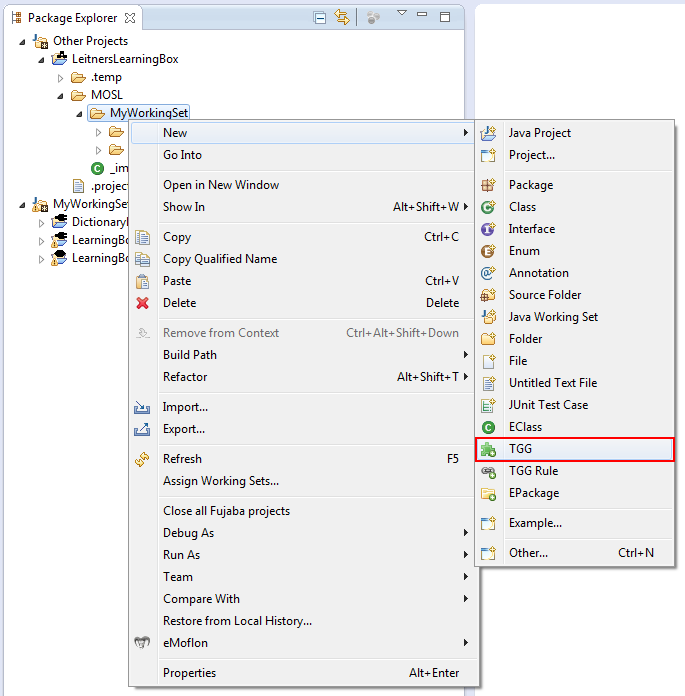
\includegraphics[width=0.8\textwidth]{eclipse_contextTGG}
  \caption{figureCaption}
  \label{fig:contextTGG}
\end{center}
\end{figure}

\item[$\blacktriangleright$] Name it \texttt{LearningBoxToDictionaryIntegration}, setting the source as \texttt{LearningBoxLanguage} and the target as
\texttt{DictionaryLanguage} (Fig.~\ref{fig:newTGG}).

\begin{figure}[htbp]
\begin{center}
  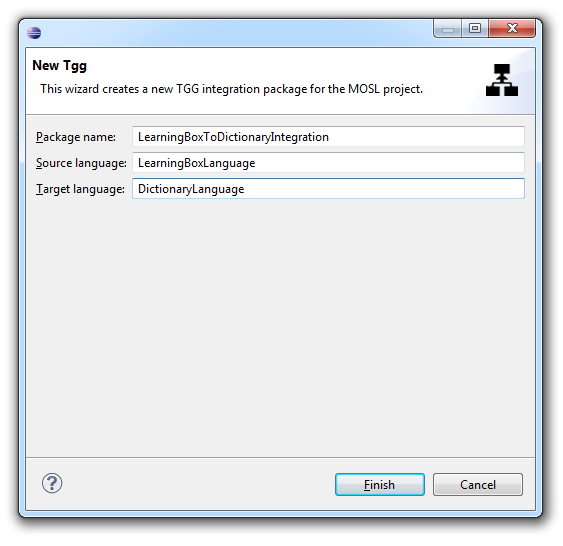
\includegraphics[width=0.8\textwidth]{eclipse_newTGG}
  \caption{figureCaption}
  \label{fig:newTGG}
\end{center}
\end{figure}

\item[$\blacktriangleright$] A new file should be active in the editor! This is the \emph{TGG Schema} which declares each \emph{correspondence type} as an
\texttt{integration class}. Press \texttt{ctrl + space} and use the auto completion to generate a new class template.

% Explain why we chose THOSE ones; Name is intetionally descriptive
\item[$\blacktriangleright$] Using the \texttt{tab} button to edit each element, name the class \texttt{BoxToDictionary}, and list the source as \texttt{Box}
and target as \texttt{Dictionary} (Fig.~\ref{fig:newTGG}).

\begin{figure}[htbp]
\begin{center}
  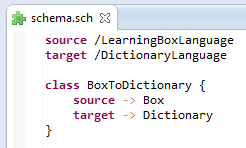
\includegraphics[width=0.4\textwidth]{eclipse_schemaFirstClass}
  \caption{figureCaption}
  \label{fig:newTGG}
\end{center}
\end{figure}

\item[$\blacktriangleright$] That's it! Your schema is now complete with connections to your \texttt{source} and \texttt{target} metamodels via a correspondence
link!

\end{itemize}
